\documentclass[10pt]{sensys-proc}

\usepackage{balance}
\usepackage{graphicx}
\usepackage{url}

\crdata{978-1-4503-1169-4}
\conferenceinfo{PhoneSense'12,} {November 6, 2012, Toronto, ON, Canada.}
\CopyrightYear{2012}

\numberofauthors{2}

\author{

\alignauthor Kasturi Rangan Raghavan, Supriyo Chakraborty, Mani Srivastava\\
	\affaddr{University of California, Los Angeles}\\
	\email{\{kasturir,supriyo,mani\}@ucla.edu}

\alignauthor Harris Teague\\
	\affaddr{Qualcomm Inc.}\\
	\email{hteague@qualcomm.com}
}

\title{textsc{Override}: A Mobile Privacy Framework for Context-Driven
Perturbation and Synthesis of Sensor Data Streams}

\begin{document}

\maketitle

\begin{abstract}
Smart phones with increased computation and sensing capabilities have spurred the growth of a new generation of context-aware apps. These apps often make judicious use of the readily-available sensor data to infer users' personal context but most do provide some useful service in return. However, sharing sensor data with apps leaves room for abuse; a malicious app can extract information that is sensitive and considered private by the user. Current approaches to mitigate the privacy concerns rely on simple user-specified policies that consist of static rules and are limited to binary access control. These rules are often conservative and lead to a sharp decline in application utility. In this paper we aim to  address the above challenge of balancing user privacy and application utility. To this end, we present \textsc{Override}: a mobile privacy framework that empowers users to control the sensor data being delivered to apps. It does so by providing apps access to perturbed or even synthetic sensor data streams. We discuss the key architectural elements of \textsc{Override} and its prototype implementation on the Android platform. We highlight its ability to give users increased transparency and control over shared sensor data, and then discuss its other secondary benefits.
\end{abstract}

\section{Introduction}
\label{sec:intro}
Increasingly, smart phone apps are context-aware and can tap into the full set of onboard sensors. These apps rely on the sensor data to infer user's context to better tailor their services resulting in increased personalization. However, sharing sensor data with apps leaves room for abuse; a malicious app can use the data to extract information that is sensitive and considered private by the user. Seemingly innocuous sensor measurements can be used to make surprisingly sensitive inferences about the user. For example, \cite{plarre:psychological, rahman:mConverse} have shown that one can reliably infer the occurrence of psychosocial stress, conversations, and smoking episodes from a simple respiration sensor
\cite{Ertin:AutoSense}. Similarly~\cite{krumm:survey} provides a survey of sensitive inferences that are possible from shared location data.

Current security mechanisms in popular mobile platforms require that applications declare the sensors that they will use during install time. However, such mechanisms provide limited ability for users to control the sensor data received by the apps. An app does not advertise the intended inferences for which it requires access to sensor data, and even if the inferences are made known the mobile platform lacks the ability to monitor the apps that may misbehave by using the data for purposes other than they claim. Finally, such a permission mechanism leaves the users with an unsatisfying binary choice on privacy: to provide no access to sensor data, or provide access at full fidelity at all times.

Such mechanisms are in stark contrast to a user's true privacy requirement which is an assurance that an app uses the sensor data appropriately for only the advertised inferences, and does not use the data for making any sensitive inferences. Moreover, the privacy requirements, may also change as a function of the user's current contextual state. For example, the user may have sensitive locations that he does not want to share with apps, but as long as the user is not in a sensitive location an app should receive location updates.

As a first step towards addressing the above challenges, we present \textsc{Override} a mobile privacy framework which provides users greater flexibility in terms of their privacy choices and better control over the flow of information to untrusted applications to meet their utility requirements. \textsc{Override} implements a secure mechanism for intercepting the access to the raw sensor data, and either replaces it with synthetic data (preserving statistical properties of the original data) or with data that has been perturbed in a context-dependent fashion according to user-specified privacy rules. For example, sensor data may be shared with different applications with different resolutions, or may be suppressed at certain times of the day, or replaced with synthetic data under certain contexts. We describe in detail the architectural elements of \textsc{Override} and provide an example of a location sharing based application scenario to demonstrate the ease of implementation using \textsc{Override}.

The design of the \textsc{Override} mechanism draws conceptual similarity with the network firewall provided via iptables in Linux. Users can configure actions on sensor data flows depending on the context and the destination application. Closest in functionality to \textsc{Override}, is Protect-My-Privacy (PMP)~\cite{pmp}. However, implemented on the iOS platform, PMP is designed for non-sensory non-time series data and focuses on tracking surreptitious and unadvertised access by applications to information sources which may have private information but which iOS allows any application to access.

The rest of the paper is organized as follows. The high-level design of the \textsc{Override} framework, and the implementation details on the Android mobile platform are presented in Section~\ref{Sec:architecture}. In Section~\ref{Sec:example} we outline an example scenario to demonstrate how \textsc{Override} can be leveraged for location privacy. Related work is summarized in Section~\ref{Sec:related} followed by a summary of the work in Section~\ref{Sec:conclusion}.

\section{The \textsc{Override} Framework}
\label{Sec:architecture}
\begin{figure}
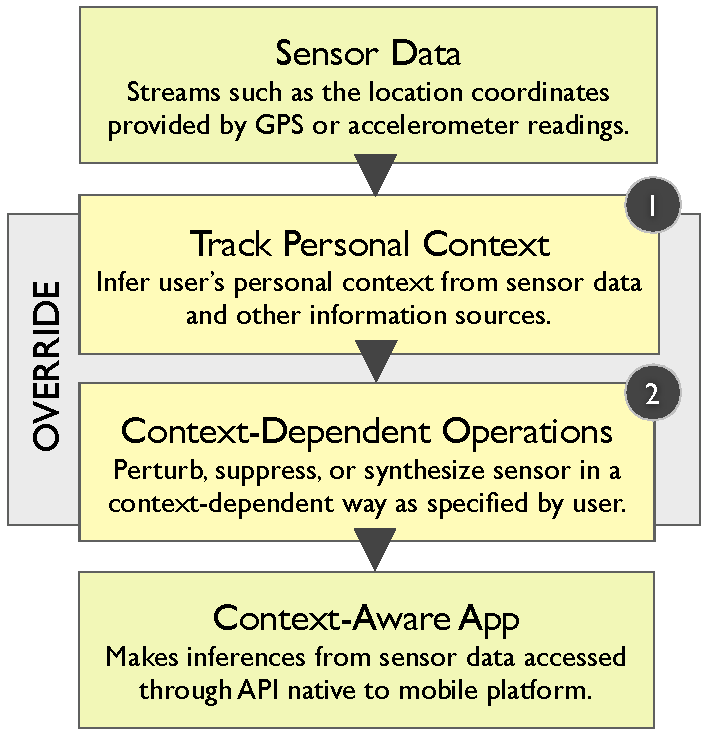
\includegraphics[width=\columnwidth]{../figures/flow5.pdf}
\caption{The key functionality of the \textsc{Override} framework.}
\label{fig:flow}
\end{figure}

In this section, we provide a high-level overview of \textsc{Override}, and then in Section~\ref{sec:implementation} discuss the details of a prototype implementation on the Android mobile platform. As visualized in Figure~\ref{fig:flow} the core functionality of \textsc{Override} is to deliver suitably processed sensor data streams to apps and facilitate context-aware privacy. This is achieved by tracking the personal context of a user (\emph{Track Personal Context}) and then applying suitable context-dependent privacy transformation on the stream (\emph{Context-Dependent Operations}). \textsc{Override} allows sensor data streams to be processed differently for each app that requests sensor data, enabling targeted control of mobile apps.

\subsection{Design Overview}

We briefly discuss tracking personal context, and then discuss broad categories of data processing operations that can be driven by personal context. More concrete applications are left for Section~\ref{Sec:example}.

\subsubsection{Tracking Personal Context.}

An external context-providing service is instantiated and left to run in the background. The service makes various contextual inferences from sensor data and from other information sources. For example, the service may make two contextual inferences: (1) user activity, and (2) indoor or outdoor. Say the former inference classifies the user's current activity into one of $\{Still, Running, Walking\}$, and that the output of the latter inference takes on one value from $\{Indoor, Outdoor, Uncertain\}$. We abstract away from the implementation details of these inferences, since \textsc{Override} does need that information. Together these inferences determine the user's personal contextual state at any point in time, and \textsc{Override} is able to track that with the help of the context-providing service.

\subsubsection{Context-Dependent Operations.}
We permit standalone, externally-implemented modules to provide \textsc{Override} with processed sensor data streams. In this way, we can readily integrate different data processing operations. Some of the mechanisms we currently support are:

\textbf{Perturbation and Noise.} We support standard mechanisms that are known to lower the quality of the sensor data signals as a means to enable privacy. For example, location coordinates can be quantized to lower the spatial resolution. Accelerometer data can be sub-sampled or otherwise filtered as a means to sanitize the signal.

\textbf{Suppression.} A special operation that allows sensor data streams to be suppressed. Compared  to perturbation which delivers lower quality sensor data to apps, suppression entirely blocks the delivery of sensor data. For instance, suppression blocks the delivery of GPS location coordinate streams, and mimics the behavior expected in the event the GPS sensor was turned off.

Sensor data streams can be perturbed or suppressed depending on the current personal context. For example, a location-aware app can be configured to receive GPS location data only when the user is outdoors. If the user is indoors, then we can suppress any location updates that would have been delivered to the app. See Section~\ref{Sec:example} for an example of context-aware sensor data processing.

\textbf{Context-Driven Sensor Data Synthesis.} Besides perturbation and suppression, a third technique we consider to facilitate privacy is sensor data synthesis. See Section~\ref{Sec:related} for prior work that has used synthetic sensor data for privacy. Here, we consider driving the synthesis of sensor data based on the current personal contextual state.

For example, we can use synthesize accelerometer data that has a certain variance to force simple  accelerometer-based activity tracking apps into making a predictable activity-level inference. Now, the variance of the synthesized sensor data can be driven by personal context--perhaps by an analogous but more sophisticated and accurate activity inference available to \textsc{Override}.

\subsection{A Prototype Android Implementation}
\label{sec:implementation}
We implemented the \textsc{Override} framework in Java within the Android mobile platform. Parts of the underlying architecture was inspired by PDroid~\footnote{Available at \url{https://play.google.com/store/apps/details?id=com.privacy.pdroid}}, an open-source framework for implementing sensor-level access control. The components of the full \textsc{Override} implementation are shown in Figure~\ref{fig:android_impl}.

In this paper, we focus on the implementation details of the \texttt{OverrideDataManager}. It makes up the main modification we have made to the Android platform, and it is the component that enables the delivery of processed sensor data streams to apps that request sensor data. We then discuss the extensibility afforded by the prototype framework that allows third parties to integrate with \textsc{Override} and provide it with processed sensor data streams. In Section~\ref{Sec:example} we discuss a location privacy example scenario enabled by such an extensible architecture.

\begin{figure}
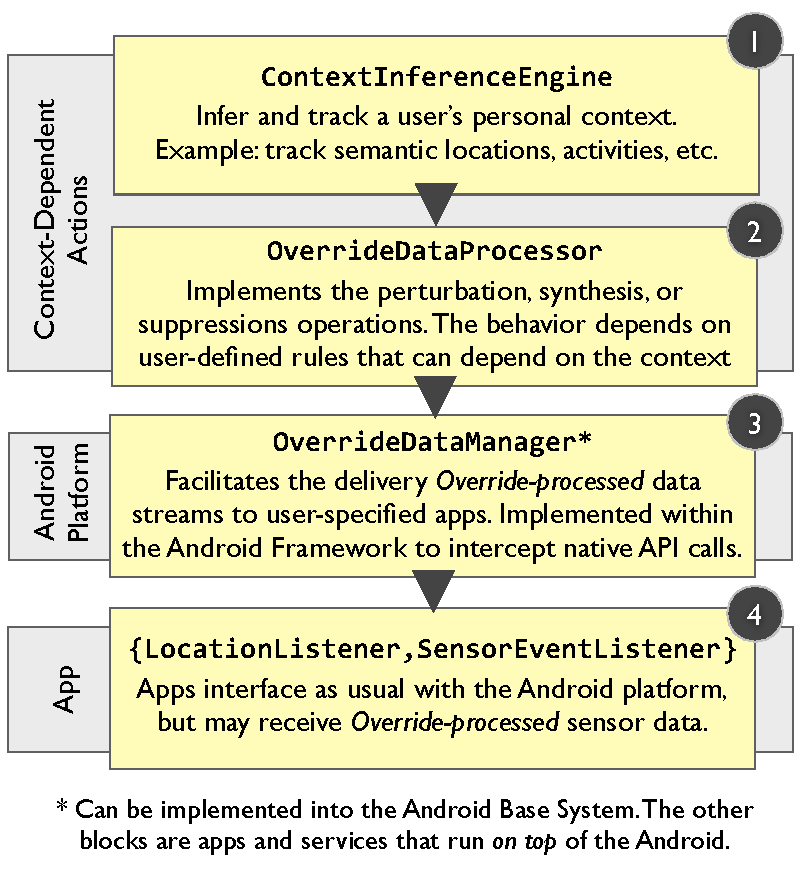
\includegraphics[width=\columnwidth]{../figures/android_impl4.pdf}
\caption{The data flow in the \textsc{Override} Android Implementation}
\label{fig:android_impl}
\end{figure}

\textbf{Replacing the Android LocationManager and SensorManager.} The Android platform maintains system services that managing the pushing of sensor data to apps. We consider the capability to process two such Android-provided sensor data streams: (1) location updates managed by the \texttt{LocationManager} and (2) \emph{sensor} updates managed by the \texttt{SensorManager}. The former provides apps that request location coordinates from GPS, WiFi-based, and cell-network sources. The latter provides apps that request accelerometer, gyroscope, and magnetic (compass) readings, and other sensors.

Android apps follow a straightforward protocol to request sensor data streams. An app first obtains a handle to one of the aforementioned \texttt{Manager} services, and then registers a data listener object with the \texttt{Manager}. Registered listeners will asynchronously receive location or sensor data as it becomes available.

We implement an \texttt{OverrideDataManager} system service, implemented alongside the existing \texttt{Manager} services inside the Android Base Framework. This new \texttt{OverrideDataManager} exposes to apps the same API as the native \texttt{Manager} services, and indeed can readily replace them. When apps attempt to obtain a handle one of the native \texttt{SensorManager} or \texttt{LocationManager} services, we deliver instead a handle to \texttt{OverrideDataManager}. In this way, we own any registered data listeners, and it enables \textsc{Override} to provide such data listeners with arbitrary processed sensor data streams.

\textbf{Standalone Services to Provide Sensor Data Streams.} Similar to the way that default Android \texttt{LocationManager} permits externally-implemented and proprietary providers of location data, our \texttt{OverrideDataManager} exposes a simple API that permits standalone Android services to report location and sensor data updates. In this way, the \texttt{OverrideDataManager} can accept perturbed or synthetic sensor data streams. This sort of functionality can be implemented by a third party developer, and distributed to users on the app-store. Each provided sensor data stream is identified by a name that is provided by the standalone service.

\textbf{Mapping Available Sensor Data Streams to Apps.} We have built a central, user-configured system service called the \texttt{OverrideSettingsManager}, and it's not shown in Figure~\ref{fig:android_impl}. This central service facilitates two decisions. First, a user will not configure all apps to receive processed sensor data, and so only those apps specifically designated in \texttt{OverrideSettingsManager} will be given a handle to the \texttt{OverrideDataManager} service that provides these apps with a processed sensor data stream. The rest of the apps will continue to operate as before and receive a handle to the default native \texttt{Manager} services. Second, since we allow standalone services to provide processed sensor data streams, the \texttt{OverrideDataManager} must choose one of these available sensor data streams to deliver to each apps. The \texttt{OverrideSettingsManager} service maintains the mapping between designated apps and the available sensor data streams.

In future versions, we imagine users will be able to specify context-dependent mappings within this service so that an app receive processed sensor data streams that depend on context. In the current prototype implementation, any context-dependent behavior and user configuration (besides the mapping maintained by \texttt{OverrideSettingsManager}) is left up to the implementation of the standalone services that provide processed sensor data streams.


\section{Semantic Locations for Privacy}
\label{Sec:example}

\begin{figure}[h]
\label{fig:semantic_places}
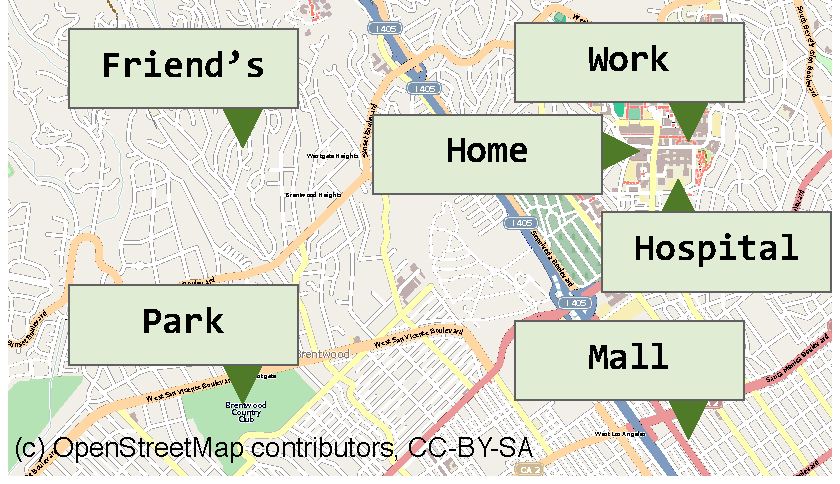
\includegraphics[width=\columnwidth]{../figures/semantic_location_3.pdf}
\caption{A set of semantic places with names and geo-tagged by the user that supplements GPS location.}
\end{figure}

Location-aware services have become very popular, increasingly so with the advent of ``check-in'' services by social networks. Naturally location is a valuable signal that's useful for pulling in local traffic, new, weather updates, and to automatically geo-tag photos when sharing them. From the user's perspective, visualizing and controlling which apps receive what location updates can promote a sense of privacy. There's a large amount of work in literature that addresses the issue of location privacy~\cite{krumm:survey}, many focus on lowering the quality of the provided location coordinates by decreasing it's resolution or adding structured noise. In this section, we demonstrate how \textsc{Override} can be leveraged to deliver custom location coordinate streams to location-aware apps as a way to facilitate location privacy.

In particular, we consider using \textsc{Override} as a mechanism to replace the conventional GPS-derived location coordinates with \emph{semantic locations}. Semantic locations are places that are personally meaningful to the user. The user maintains a geo-tagged set of semantic locations; see Figure~\ref{fig:semantic_places} for an example. GPS-derived location coordinates can be used to infer the user's current semantic location.

The primary privacy benefit that results from sharing semantic locations is because the shared locations are meaningful to the user and they are explicitly allowed to be shareable with an app. When the user configures \textsc{Override} to deliver semantic locations to apps in lieu of GPS-derived location, these apps will being to receive location coordinates that jump between the user's semantic locations as the user moves between them. If the user is not in a valid semantic location or if that semantic location is not allowed to be shared with an app, then \textsc{Override} can be setup to suppress location updates.

The uses of \textsc{Override} are not limited to just the above example. Note that at any one time there can be available location providers each implemented as standalone services that report differently processed location coordinate streams to the \texttt{OverrideDataManager}. Another location provider may incorporate different location privacy mechanisms such as providing a perturbed GPS signal. For example, a location-aware weather application can be configured to receive location coordinates have a zip-code level resolution. At that level the weather app is able to maintain its ability to figure out the user's locality, but at that low resolution the app is unable to make other sensitive inferences that often require more fine-grained location data. More straightforward location privacy mechanisms such as geo-fencing apps to receive location updates only within a certain geographical area can also be realized. In this way, \textsc{Override} can serve as a location-privacy platform that empowers users to to curb apps' ability to make unadvertised and possibly sensitive inferences. We want to implement in the future more sophisticated context-driven suppression mechanisms such as that in~\cite{Gotz:MaskIt}.

\textsc{Override} can also be leveraged to address other privacy concerns besides location privacy. In our implementation we also have the ability to override the others sensors that exist in Android. In particular, the onboard accelerometer sensor is a popularly used sensor that is used by many fitness and wellness apps as a means track activity levels. Recently, we have seen some work that revealed a user's keyboard strokes on the phone's soft keyboard can be deciphered from capturing only the accelerometer data from the onboard sensors~\cite{}. To alleviate such concerns, \textsc{Override} can be configured to suppress accelerometer data to all apps whenever the soft keyboard is visible on the screen. As an alternative to suppression, we can configure \textsc{Override} to to add Gaussian noise to the accelerometer data whenever the software keyboard is visible.

We will now describe at a high level an instantiation of \textsc{Override} to incorporate semantic location updates delivered to apps. We follow the proposed Android architecture from Section~\ref{sec:implementation}; in particular, following the component-level description in Figure~\ref{fig:android_impl}. Consider the semantic location inferences are implemented by a standalone Android service. This service provides a UI to allow the user to maintain the list of geo-tagged semantic locations, and it reports to the \texttt{OverrideDataManager} the user's semantic location as it is changes over time. In this system, we have combined the functionality of the \texttt{ContextInferenceEngine} and \texttt{OverrideDataProcessor} blocks from Figure\ref{fig:android_impl} into a monolithic standalone service. We can think of the semantic locations as a context-dependent perturbation operation on the original GPS-derived location coordinates. This service periodically pushes location updates in the form of (latitude, longitude) coordinates to the \texttt{OverrideLocationManager}. Finally, a separate UI as provided by the\texttt{OverrideSettingsManager} allows the user to specify which app should receive semantic location updates in lieu of GPS-derived location. With the aforementioned configuration in place, \textsc{Override} will ensure that the designated apps will receive the semantic location updates.

\subsection{More Comprehensive Location Providers}
Higher-level contextual inferences can often supplement sensor data streams, making them more accurate or more available. For example, GPS is a very accurate sensor of location. This sensor works great when outdoors, but the signal is often unavailable indoors. To combat this weakness, the research community have proposed various effective alternatives that can infer location when GPS is not available. For instance, in the previous section we discussed the inference of semantic locations using GPS as the primary sensor. However, these semantic locations can also be inferred  via WiFi and Bluetooth landmarks~\cite{Kim:PlaceSens,Ananthanarayanan:BlueFi}, and interestingly such a location inference is often most useful indoors. In this sense, GPS-derived location when supplemented with semantic locations can serve as a more comprehensive location provider. In this way, we can let \textsc{Override} supplement GPS-derived location so that inferred semantic locations are delivered whenever GPS is unavailable.

Moreover, an intelligently implemented system can leverage the availability of semantic location, allowing the GPS to be opportunistically turned off. And since the power-hungry GPS sensor is less frequently needed, this can contribute to improved battery life in the long run. We leave a thorough quantitative evaluation of such benefits to future work.

\section{Related Work}
\label{Sec:related}
It is well known that mobile phone sensor data can be used to make a rich set of inferences about personal context and behavior. More recent work in this space have even explored using collaborative inference algorithms and information fusion for improved inferences~\cite{Miluzzo:DarwinPhones}. There's been much work on designing mobile platforms that have built-in services that can provide apps with \emph{contextual inferences} directly. This line of thinking is a natural progression of mobile platform design, see~\cite{Raento:ContextPhones} or more recently~\cite{Chu:CondOS} for an overview of two architectures. However, current mobile platforms do not incorporate such architectures, and apps must resort to operating on sensor data, even if internally a context-providing library is used to make appropriate inferences.

Sharing \emph{contexts} with apps instead of the sensor data is useful for controlled context release. This way, the mobile platform can inform the user more precisely what is being shared, it increases the transparency of what's shared and it is useful for privacy. However, many existing apps do not make use of context-providing libraries, and neither context-providing libraries nor typical context-aware apps expose any user interface that allows users to control the types of inferences being made from sensor data. Unless current mobile platforms incorporate provide high-level context directly, apps will remain to operate directly on sensor data. The work in this paper presents a framework that's practical to implement on current mobile platforms and does not require that apps use a special context-providing library. This work represents a solution that enables users to control the the many existing apps that operate directly on sensor data.

There is prior work on tracking when and what sensor data is accessed, providing capabilities beyond what exists in the current mobile platforms. Some such systems allow the user to limit an individual app's access to sensor data, or let users configure it to send a fixed synthetic value~\cite{Beresford:MockDroid,Enck:TaintDroid}. These works we classify as basic access control and information flow mechanisms applied to sensor data sources. They are limited to providing users with static policies. For example, \cite{Beresford:MockDroid} enable a user to setup a rule such that an app always receives a fixed location value. The work presented in this paper is complimentary to previous work. To the best of our knowledge, we have not seen before the idea of using personal context to \emph{drive} the perturbation or synthesis of sensor data. Other approaches taken for privacy consider suppressing \emph{sensitive} contexts and some systems even attempt to block \emph{inference of sensitive contexts}~\cite{Gotz:MaskIt}, but these are just studies and they are not implemented as true mobile frameworks. We imagine system architectures such as \textsc{Override} can facilitate the aforementioned privacy mechanisms, but we leave a thorough evaluation to future work.

\section{Summary}
\label{Sec:conclusion}
We presented \textsc{Override}, a privacy framework that allows users to exercise fine-grained context-aware control over the sensory data being shared with various untrusted applications. \textsc{Override} provides this functionality by intercepting the sensor data requests from applications and applying user specified privacy-preserving transformations such as perturbation and suppression of data, or synthesis of data streams before sharing. We provided a prototype implementation of the framework and used a location sharing based application scenario to illustrate the ease of application development using the framework.

\balance
\bibliographystyle{abbrv}
\bibliography{override}
\end{document}
